\section{機器配置 $\cdot$ 放熱面の決定}

\subsection{仮定}
\begin{enumerate}
  \item 各空間内では同一温度とする
  \item バルクヘッドは断熱材とする。
  \item 構造重量は機器の10\%とし、重心は面の中心とする。
  \item 電気機械軽装重量は機器の7\%とし、重心は面の中心とする。
  \item 構造重量は機器の7\%とし、重心は面の中心とする。
  \item ヒドラジンスラスタは$ \pm SUN$面中央に配置する。
  \item 面、バルクヘッドの面圧は0として計算する
  \item 座標系、空間の名前を下図のようにとる。
\end{enumerate}

\begin{figure}[H]
  \caption{衛星断面(水平方向)}
\begin{center}
  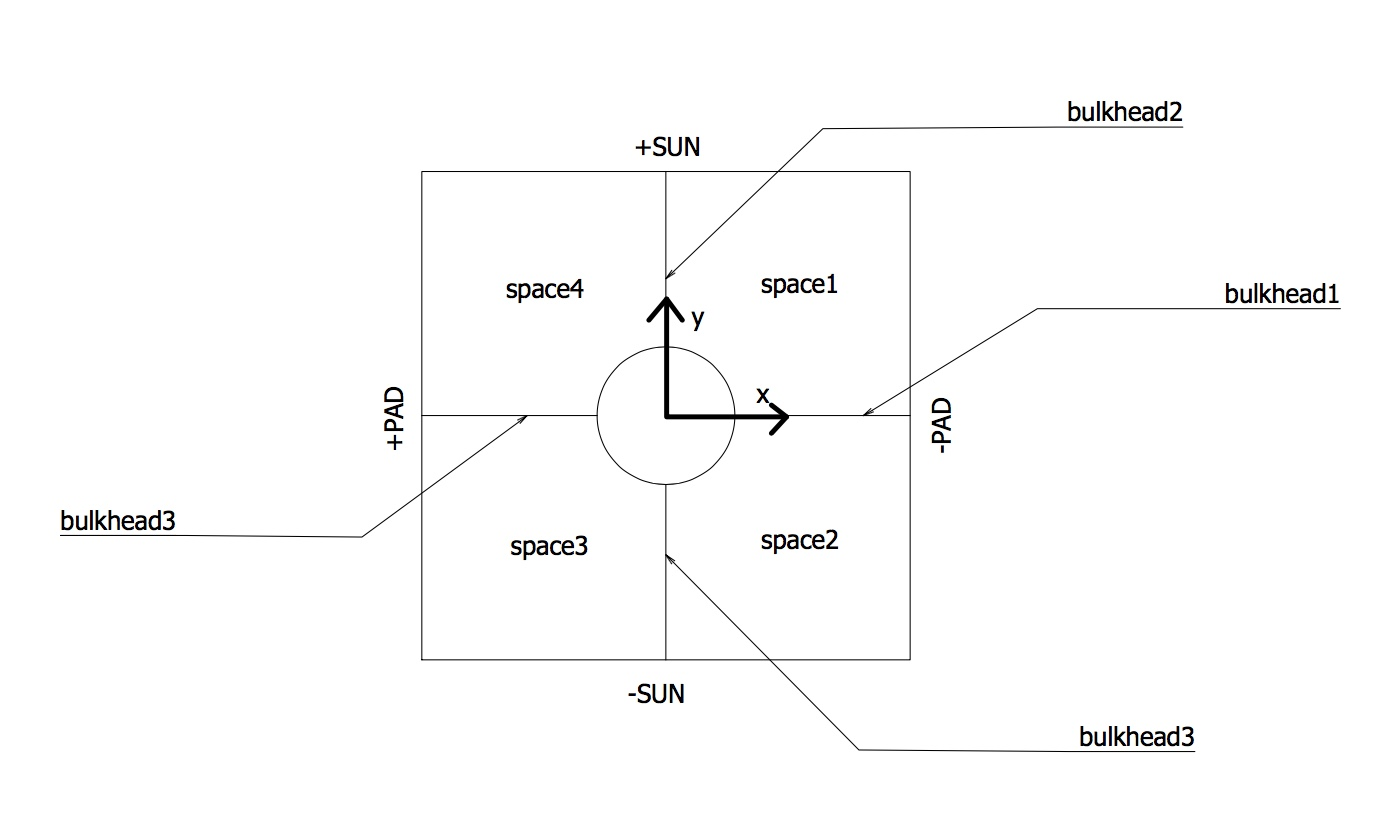
\includegraphics[scale=0.5]{satelite1.eps}
\end{center}
\end{figure}

\begin{figure}[H]
  \caption{衛星断面(鉛直方向)}
\begin{center}
  \includegraphics[scale=0.3]{satelite2.eps}
\end{center}
\end{figure}
\newpage

\subsection{機器配置図 $\cdot$ 搭載機器表 $\cdot$ 重心、重量表}
機器配置図,搭載機器表、重心、重量表は以下のようにした。
\begin{figure}[H]
  \caption{機器配置図(水平方向)}
\begin{center}
  \includegraphics[scale=0.8]{satelitetop.eps}
\end{center}
\end{figure} \newpage

\begin{figure}[H]
  \caption{機器配置図(鉛直方向)}
\begin{center}
  \includegraphics[scale=0.8]{sateliteside.eps}
\end{center}
\end{figure} \newpage

\begin{table}[H]
\caption{搭載機器表}
\setlength{\tabcolsep}{.5zw}
\begin{tabularx}{55zw}{c|c c c C C C c } \hline
  & 機器名 & 寸法[cm] & 重量[kg] & 消費電力[W] & 発熱量[W] & 許容温度$[^ \circ C]$ & 搭載面\\ \hline
  & \shortstack{uplinkパラボラアンテナ \\ (Sバンド)} & \o 70 & 5 & 0 & 0 & 10-40 & +TAR外\\ \cline{2-8}
  & \shortstack{uplinkパラボラアンテナ \\ (Kaバンド)} & \o 150 & 23 & 0 & 0 & 10-40 & +TAR外\\ \cline{2-8}
  & \shortstack{downlinkパラボラアンテナ \\ (Sバンド)} & \o 80 & 6 & 0 & 0 & 10-40 & +TAR外\\ \cline{2-8}
  & \shortstack{downlinkパラボラアンテナ \\ (Kaバンド)} & \o 160 & 26 & 0 & 0 & 10-40 & +TAR外\\ \cline{2-8}
  \raisebox{2.5\normalbaselineskip}[0pt][0pt]{ミッション機器}
  & アンテナタワー & & 70 & 0 & 0 & -45-65 & +TAR外\\ \cline{2-8}
  & Kaバンド中継機 & $138 \times 70 \times 20$ & 180 & 867 & 694 & 5-40 & BH3/SP2\\ \cline{2-8}
  & Sバンド中継機 & $70 \times 70 \times 70$ & 60 & 330 & 264 & 5-40 & BH1/SP4 \\ \hline

  & アースセンサ & $12 \times 17 \times 13$ & 25 & 6 & 6 & 0-50 & +TAR外\\ \cline{2-8}
  & $サンセンサ \times 2$ & $12 \times 43 \times 13$ & $4.5 \times 2$ & $6 \times 2$
  & $6 \times 2$ & 0-50 & $\pm$ SUN外\\ \cline{2-8}
  & IRU & $30 \times 38 \times 30$ & 22 & 10 & 10 & 0-40 & -TAR/SP1\\ \cline{2-8}
  & AOCE & $20 \times 15 \times 7$ & 10 & 50 & 50 & -5-40 & -TAR/SP3\\ \cline{2-8}
  & リアクションホイール & $30 \times 30 \times 10$ & 24 & 60 & 60 & 0-45 & -TAR/SP4 \\ \cline{2-8}
  & TT\&Cユニット & $80 \times 60 \times 20$ & 60 & 35 & 35 & 0-50 & -TAR/SP1\\ \cline{2-8}
  & オンボード計算機 & $40 \times 26 \times 12$ & 20 & 120 & 120 & -5~40 & -TAR/SP4\\ \cline{2-8}
  \raisebox{.5\normalbaselineskip}[0pt][0pt]{バス機器}
  & ヒドラジンスラスタ$\times 2$ &  & $10 \times 2$ &  &  & 9-40 & $\pm$SUN外 \\ \cline{2-8}
  & 太陽電池パドル$\times 2$ &  & $77 \times 2$ &  &  &  & $\pm$PAD外 \\ \cline{2-8}
  & パドル駆動モータ$\times 2$ & $19 \times 20 \times 34$ & $13 \times 2$ & $10 \times 2$ & $10 \times 2$ & 0-40 & $\pm$PAD/SP2,4 \\ \cline{2-8}
  & バッテリ$\times 2$ & $35 \times 25 \times 20$ & $25 \times 2$ &  & $117 \times 2$ & 5-20 & $\pm$PAD/SP1,3  \\ \cline{2-8}
  & 電源制御部$\times 2$ & $20 \times 30 \times 20$ & $10 \times 2$ & $25 \times 2$ & $25 \times 2$ & 0-40 & $\pm$PAD/SP2,4\\ \hline

  & ヒドラジンタンク$\times 2$ & r=35(球) & $16.92 \times 2$ & 0 & 0 & 9-40 & バルクヘッド \\ \cline{2-8}
  \raisebox{.5\normalbaselineskip}[0pt][0pt]{タンク系}
  & アポジタンク & r=58(球) & 155.1 & 0 & 0 & 9-40 & スラストチューブ \\ \hline

\end{tabularx}
\end{table}
\newpage

\begin{table}[H]
\caption{重心計算表}
\setlength{\tabcolsep}{.5zw}
\begin{tabularx}{55zw}{c|c|C C C C C|C C C c c c} \hline
面 & 機器名 & \shortstack{機器 \\ 重量 \\ $[kg]$} & \shortstack{構造 \\ 重量 \\ $[kg]$} & \shortstack{計装 \\ 重量 \\ $[kg]$}
 & \shortstack{マー \\ ジン \\ $[kg]$} & \shortstack{面 \\ 重量 \\ $[kg]$}
 & \shortstack{x \\ $[cm]$} & \shortstack{y \\ $[cm]$} & \shortstack{z \\ $[cm]$}
 & \shortstack{$M_x$ \\ $[kg \cdot cm]$} & \shortstack{$M_y$ \\ $[kg \cdot cm]$} & \shortstack{$M_z$ \\ $[kg \cdot cm]$} \\ \hline

 & アンテナ類 & 130.00 & 13.00 & 9.10 & 10.65 & 32.747 & 0 & 0 & 200 & 0 & 0 & 2600 \\
 & アースセンサ & 25.00 & 2.50 & 1.75 & 2.05 & 6.30 & 143 & -150 & 157 & 3575 & -3750 & 3912 \\
 \raisebox{1.0\normalbaselineskip}[0pt][0pt]{+TAR}
 & 面 & 39.05 & & & & & 0 & 0 & 75 & 0 & 0 & 2930 \\ \hline

 & IRU & 22.00 & 2.20 & 1.54 & 1.80 & 5.54 & 65 & 135 & 19 & 1421 & 2970 & 418.0 \\
 & TT\&Cユニット & 60.0 & 6.00 & 4.20 & 4.91 & 15.11 & 95 & 53 & 10 & 5700 & 3180 & 600 \\
 & AOCE & 10.00 & 1.00 & 0.70 & 0.82 & 2.52 & -58 & -92 & 3 & -581 & -920 & 35 \\
 \raisebox{1.0\normalbaselineskip}[0pt][0pt]{-TAR}
 & リアクションホイール & 24.0 & 2.40 & 1.68 & 1.96 & 6.05 & 105 & -45 & 5 & 2520 & -1080 & 120 \\
 & オンボード計算機 & 20.00 & 2.00 & 1.40 & 1.64 & 5.04 & 80 & -80 & 6 & 1608 & -1600 & 120 \\
 & 面 & 34.26 &  &  &  &  & 0 & 0 & 75 & 0 & 0 & 2569 \\ \hline

 & サンセンサ & 4.50 & 0.45 & 0.32 & 0.37 & 1.13 & 77 & 166 & 75 & 344 & 747 & 338 \\
 & ヒドラジンスラスタ & 10.0 & 1.00 & 0.70 & 0.82 & 2.52 & 0 & 180 & 75 & 0 & 1800 & 750 \\
 \raisebox{1.0\normalbaselineskip}[0pt][0pt]{+SUN}
 & 面 & 3.65 & & & & & 0.0 & 160 & 75 & 0 & -584 & 274 \\ \hline

 & サンセンサ & 4.50 & 0.45 & 0.32 & 0.37 & 1.13 & -77 & -166 & 75 & -344 & -747 & 338 \\
 & ヒドラジンスラスタ & 10.0 & 1.00 & 0.70 & 0.82 & 2.52 & 0 & -180 & 75 & 0 & -1800 & 750\\
 \raisebox{1.0\normalbaselineskip}[0pt][0pt]{-SUN}
 & 面 & 3.65 & & & & & 0 & -160 & 75 & 0 & -584 & 274 \\ \hline

 & 太陽電池パドル & 77.0 & 7.70 & 5.39 & 6.30 & 19.40 & -400 & 0 & 75 & -30800 & 0 & 5775 \\
 & パドル駆動モータ & 13.0 & 1.30 & 0.91 & 1.07 & 3.28 & -151 & 10 & 75 & -1957 & 130 & 975 \\
 & バッテリ & 25.00 & 2.50 & 1.75 & 2.05 & 6.30 & -148 & -133 & 10 & -3688 & -3313 & 250 \\
 \raisebox{1.0\normalbaselineskip}[0pt][0pt]{+PAD}
 & 電源制御部 & 10.0 & 1.00 & 0.70 & 0.82 & 2.52 & -150 & 115 & 10 & -1500 & 1150 & 100 \\
 & 面 & 31.50 & & & & & -160 & 0 & 75 & -5038 & 0 & 23612 \\ \hline

 & 太陽電池パドル & 77.0 & 7.70 & 5.39 & 6.30 & 19.40 & 400 & 0 & 75 & 30800 & 0 & 5775 \\
 & パドル駆動モータ & 13.0 & 1.30 & 0.91 & 1.07 & 3.28 & 151 & -10 & 75 & 1957 & -130 & 975 \\
 & バッテリ & 25.00 & 2.50 & 1.75 & 2.05 & 6.30 & 148 & 133 & 10 & 3688 & 3313 & 250 \\
 \raisebox{1.0\normalbaselineskip}[0pt][0pt]{-PAD}
 & 電源制御部 & 10.0 & 1.00 & 0.70 & 0.82 & 2.52 & -150 & -115 & 10 & 1500 & -1150 & 100 \\
 & 面 & 31.50 & & & & & -160 & 0 & 75 & -5038 & 0 & 23612 \\ \hline

 & Sバンド中継機 & 60.0 & 6.00 & 4.20 & 4.91 & 15.11 & 100 & -10 & 45 & 6000 & -600 & 2700 \\
 \raisebox{0.5\normalbaselineskip}[0pt][0pt]{BH1}
 & 面 & 15.11 & & & & & 80.00 & 0 & 75 & 1209 & 0 & 1134 \\ \hline

 & ヒドラジンタンク & 16.92 & 1.69 & 1.19 & 1.39 & 4.26 & 0 & 110 & 75 & 0 & 1862 & 1269 \\
 & ヒドラジン & 169.24 & & & & & 0.0 & 110 & 75.0 & 0.0 & 18616 & 12693 \\
 \raisebox{0.5\normalbaselineskip}[0pt][0pt]{BH2}
 & 面 & 15.11 & & & & & 80.00 & 0.0 & 75 & 0 & 341 & 320 \\ \hline

 & Kaバンド中継機 & 180.0 & 18.00 & 12.6 & 14.74 & 45.34 & -100 & 10 & 69 & -18000 & 1800 & 12420 \\
 \raisebox{0.5\normalbaselineskip}[0pt][0pt]{BH3}
 & 面 & 45.34 & & & & & -80 & 0 & 75 & -3627 & 0 & 3401 \\ \hline

 & ヒドラジンタンク & 16.92 & 1.69 & 1.19 & 1.39 & 4.26 & 0 & -110 & 75 & 0 & 1862 & 1269 \\
 & ヒドラジン & 169.24 & & & & & 0 & -110 & 75 & 0 & -18616 & 12693 \\
  \raisebox{0.5\normalbaselineskip}[0pt][0pt]{BH4}
 & 面 & 15.11 & & & & & 80 & 0 & 75 & 0 & -341 & 320 \\ \hline

 & アポジタンク & 155.1 & 15.5 & 10.9 & 12.7 & 39.1 & 0 & 0 & 75 & 0 & 0 & 11634 \\
 & 過塩素酸アンモニウム & 1551.2 & & & & & 0 & 0 & 75 & 0 & 0 & 116340 \\
 \raisebox{0.5\normalbaselineskip}[0pt][0pt]{TT}
 & 面 & 39.08 & & & & & 0 & 0 & 75 & 0 & 0 & 2930 \\ \hline
\end{tabularx}
\end{table}
\newpage

\subsection{重心の位置}
重心の値は以下の通りとなる.
\begin{equation}
  x = 1.27 \times 10 ^ {-5}
\end{equation}
\begin{equation}
  y = -4.71 \times 10 ^ {-5}
\end{equation}

\subsection{熱計算と放熱面の設計}
Chapter3より,PAD面は季節によって放熱能力が大きくするので,
PAD面はプラスマイナス断熱材とする.また,+TAR面には前の設計図よりたくさんの
機器が取り付けられているので放熱面にはSUN面と-TAR面を用いる.さらにここでは
空間温度は$20^\circ$付近であり,各機器の許容温度内に収められるように
設計することを考える.

\subsubsection{空間1}
\begin{table}[H]
  \begin{center}
  \caption{空間1}
  \scalebox{1}[1]{
  \begin{tabular}{|c|c|c|} \hline
    機器名 &  発熱量 & 許容温度 \\ \hline
  TT\&C ユニット
  & 35W
  & 0 〜 ${50}^\circ\mathrm{C}$\\

  サンセンサ
  & 3W
  & 0 〜 ${50}^\circ\mathrm{C}$\\

  バッテリ
  & 113.925W
  & 5 〜 ${20}^\circ\mathrm{C}$\\

  IRU
  & 10W
  & 0 〜 ${40}^\circ\mathrm{C}$\\

  アンテナ類
  & 0W
  & 10 〜 ${40}^\circ\mathrm{C}$\\

  ヒドラジンスラスタ
  & 0W
  & 9 〜 ${40}^\circ\mathrm{C}$\\

  ヒドラジンタンク
  & 0W
  & 9 〜 ${40}^\circ\mathrm{C}$\\

  太陽電池パドル
  & 0W
  &  熱計算不要\\ \hline

  合計発熱量
  & 161.925W
  & \\\hline
  \end{tabular}
  }
\end{center}
\end{table}

+SUN面での放熱能力を考える.春秋分の時に${20}^\circ\mathrm{C}$
に保つとして、必要な放熱面積Sは
\begin{eqnarray}
  S=\frac{161.925}{248.5}=0.652m^2<\text{+PAD面の面積の半分}
\end{eqnarray}
放熱面積がこのとき,夏至の温度は
\begin{eqnarray}
  (\epsilon\sigma T^4 -79.34)S=Q\\
  T =(\frac{\frac{161.925}{0.652}+79.343}
  {0.8\times5.67\times10^{-8}})^{\frac{1}{4}}=291.54K
\end{eqnarray}
よって許容範囲温度範囲内である.

\subsubsection{空間2}

\begin{table}[H]
  \begin{center}
  \caption{空間2}
  \scalebox{1}[1]{
  \begin{tabular}{|c|c|c|} \hline
    機器名 &  発熱量 & 許容温度 \\ \hline

  パドル駆動モータ
  & 5W
  & 0 〜 ${40}^\circ\mathrm{C}$\\

  電源制御部
  & 12.5W
  & 0 〜 ${40}^\circ\mathrm{C}$\\

  Ka バンド中継器
  & 693.6W
  & 5 〜 ${40}^\circ\mathrm{C}$\\

  アンテナ類
  & 0W
  & 10 〜 ${40}^\circ\mathrm{C}$\\

  ヒドラジンスラスタ
  & 0W
  & 9 〜 ${40}^\circ\mathrm{C}$\\

  ヒドラジンタンク
  & 0W
  & 9 〜 ${40}^\circ\mathrm{C}$\\

  太陽電池パドル
  & 0W
  &  熱計算不要\\ \hline

  合計発熱量
  & 711.1W
  & \\\hline
  \end{tabular}
  }
\end{center}
\end{table}

+SUNと-TAR面を放熱面として面積を同一とすると
春秋分の時の温度を${20}^\circ\mathrm{C}$として
必要な放熱面積は
\begin{eqnarray}
  S=\frac{711.1}{248.5\times2}=1.43<2.4
\end{eqnarray}
この時の夏至の平衡温度は
\begin{eqnarray}
  (\epsilon\sigma T^4\times2 -79.34\times2)S=Q\\
  T =(\frac{\frac{711.1}{1.43}+79.343\times2}
  {0.8\times5.67\times10^{-8}\times2})^{\frac{1}{4}}=291.6K
\end{eqnarray}
となり許容温度範囲内である.

\subsubsection{空間3}
\begin{table}[H]
  \begin{center}
  \caption{空間3}
  \scalebox{1}[1]{
  \begin{tabular}{|c|c|c|} \hline
    機器名 &  発熱量 & 許容温度 \\ \hline

  サンセンサ
  & 3W
  & 0 〜 ${50}^\circ\mathrm{C}$\\

  バッテリ
  & 113.925W
  & 0 〜 ${40}^\circ\mathrm{C}$\\

  AOCE
  & 50W
  & $-5$ 〜 ${40}^\circ\mathrm{C}$\\

  アンテナ類
  & 0W
  & 10 〜 ${40}^\circ\mathrm{C}$\\

  ヒドラジンスラスタ
  & 0W
  & 9 〜 ${40}^\circ\mathrm{C}$\\

  ヒドラジンタンク
  & 0W
  & 9 〜 ${40}^\circ\mathrm{C}$\\

  太陽電池パドル
  & 0W
  &  熱計算不要\\ \hline

  合計発熱量
  & 166.925W
  & \\\hline
  \end{tabular}
  }
\end{center}
\end{table}
放熱を-SUN面として春秋分時に${20}^\circ\mathrm{C}$となる
放熱面積は
\begin{eqnarray}
  S=\frac{166.925}{248.5}=0.67<2.4
\end{eqnarray}
この放熱面積で、夏至の時の温度を計算すると
\begin{eqnarray}
  (\epsilon\sigma T^4 -79.34)S=Q\\
  T =(\frac{\frac{166.925}{0.67}+79.343}
  {0.8\times5.67\times10^{-8}})^{\frac{1}{4}}=291.7K
\end{eqnarray}
よって許容温度範囲内となる.

\subsubsection{空間4}

\begin{table}[H]
  \begin{center}
  \caption{空間4}
  \scalebox{1}[1]{
  \begin{tabular}{|c|c|c|} \hline
    機器名 &  発熱量 & 許容温度 \\ \hline

  パドル駆動モータ
  & 5W
  & 0 〜 ${40}^\circ\mathrm{C}$\\

  電源制御部
  & 12.5W
  & 0 〜 ${40}^\circ\mathrm{C}$\\

  Sバンド中継器
  & 264W
  & $5$ 〜 ${40}^\circ\mathrm{C}$\\

  リアクションホイール
  & 60W
  & 0 〜 ${45}^\circ\mathrm{C}$\\

  オンボード計算機
  & 120W
  & -5 〜 ${40}^\circ\mathrm{C}$\\

  ヒドラジンタンク
  & 0W
  & 9 〜 ${40}^\circ\mathrm{C}$\\

  アースセンサ
  & 6W
  & 0 〜 ${50}^\circ\mathrm{C}$\\

  アンテナ類
  & 0W
  & 10 〜 ${40}^\circ\mathrm{C}$\\

  ヒドラジンスラスタ
  & 0W
  & 9 〜 ${40}^\circ\mathrm{C}$\\

  ヒドラジンタンク
  & 0W
  & 9 〜 ${40}^\circ\mathrm{C}$\\

  太陽電池パドル
  & 0W
  &  熱計算不要\\ \hline

  合計発熱量
  & 467.5W
  & \\\hline
  \end{tabular}
  }
\end{center}
\end{table}
放熱を-SUN面と-TAR面して春秋分時に${20}^\circ\mathrm{C}$となる
放熱面積は
\begin{eqnarray}
  S=\frac{467.5}{248.5\times2}=0.94<2.4
\end{eqnarray}
この面積の時の夏至の時の温度は
\begin{eqnarray}
  (\epsilon\sigma T^4\times2 -79.34\times2)S=Q\\
  T =(\frac{\frac{467.5}{0.94}+79.343\times2}
  {0.8\times5.67\times10^{-8}\times2})^{\frac{1}{4}}=291.6K
\end{eqnarray}
となり許容温度範囲内となる.

\subsubsection{空間$1 \sim 4$の平衡温度}
各空間の平均温度をまとめると以下の通り.
\begin{table}[H]
  \begin{center}
  \caption{各空間の平衡温度}
  \scalebox{1}[1]{
  \begin{tabular}{|c|c|c|} \hline
    空間 &  春秋分 & 夏至 \\ \hline

  空間1
  & ${20}^\circ\mathrm{C}$
  & ${18.35}^\circ\mathrm{C}$\\

  空間2
  & ${20}^\circ\mathrm{C}$
  & ${18.45}^\circ\mathrm{C}$\\

  空間3
  & ${20}^\circ\mathrm{C}$
  & ${18.55}^\circ\mathrm{C}$\\

  空間4
  & ${20}^\circ\mathrm{C}$
  & ${18.45}^\circ\mathrm{C}$\\\hline
  \end{tabular}
  }
\end{center}
\end{table}
